\documentclass[intlimits, 12pt, unicode]{beamer}

\usepackage[T2A]{fontenc}
\usepackage[utf8]{inputenc}
\usepackage[russian]{babel}

\usepackage{graphicx}

\usepackage{amssymb}
\usepackage{amsthm}
\usepackage{diagbox}
\usepackage{beamerthemesplit}
\usepackage{xcolor,colortbl}

\usetheme{Warsaw}

\makeatletter
\setbeamertemplate{headline}{%
    \leavevmode%
    \begin{beamercolorbox}[wd=.5\paperwidth,ht=2.5ex,dp=1.5ex]{section in head/foot}%
        \hfill\strut\insertsectionhead\hspace{.5em}\mbox{}%
    \end{beamercolorbox}%
    \begin{beamercolorbox}[wd=.5\paperwidth,ht=2.5ex,dp=1.5ex]{subsection in head/foot}%
        \mbox{}\hspace{.5em}\strut\insertsubsectionhead\hfill%
    \end{beamercolorbox}%
}
\makeatother

\usefonttheme[onlymath]{serif}

\setbeamerfont{institute}{size=\normalsize}

\setbeamercolor{bluetext_color}{fg=blue}
\newcommand{\bluetext}[1]{{\usebeamercolor[fg]{bluetext_color}#1}}

\setbeamertemplate{navigation symbols}{}
\setbeamertemplate{caption}[numbered]

\graphicspath{{figures/}}
\DeclareGraphicsExtensions{.pdf,.png,.jpg}

\newtheorem{ru_def}{Определение}
\renewenvironment{definition}{\begin{ru_def}}{\end{ru_def}}

\setbeamercovered{transparent}

\title[Система компьютерного зрения \dots \nobreak\hfill \insertframenumber\,/\,\inserttotalframenumber]{Система компьютерного зрения для детектирования опасных ситуаций на производстве}
\author{Фомин~Никита~Алексеевич,~М26 группа}
\institute{Научный руководитель: к.ф.-м.н.,~доцент~Солдатенко~Илья~Сергеевич \\
    Тверской~государственный~университет \\
	Факультет~прикладной~математики~и~кибернетики \\
	Кафедра~информатики~и~информационных~технологий \\
}
\date{
	Тверь ---
	2024
}

\begin{document}
	\maketitle

	%\begin{frame}
	%	\frametitle{Содержание}
    %    \tableofcontent
	%\end{frame}

	\section{Постановка задачи}

\begin{frame}
    \frametitle{Постановка задачи}
    \begin{figure}
        \centering
        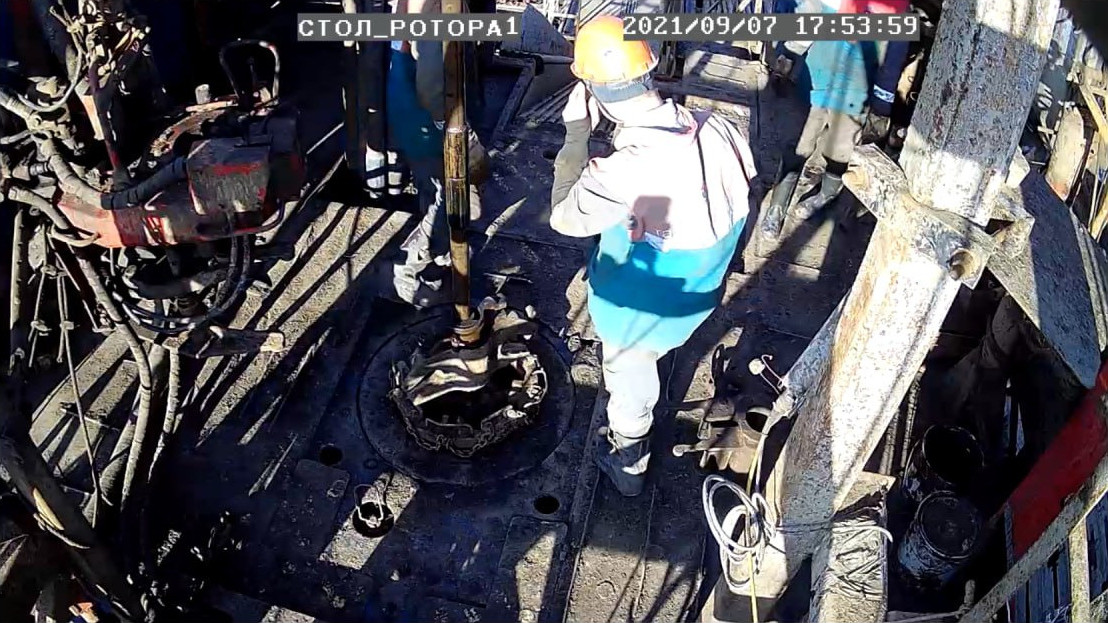
\includegraphics[width=1.0\textwidth,keepaspectratio]{problem_formulation_1}
    \end{figure}
\end{frame}

\begin{frame}
    \frametitle{Постановка задачи}
    \begin{figure}
        \centering
        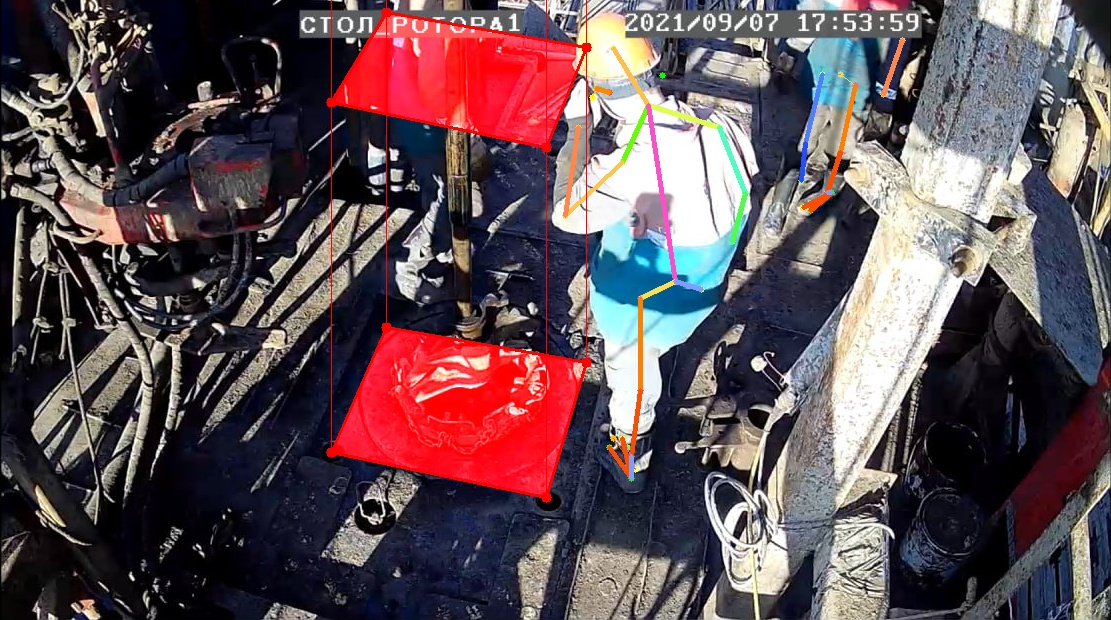
\includegraphics[width=1.0\textwidth,keepaspectratio]{problem_formulation_2}
    \end{figure}
\end{frame}

\begin{frame}
    \frametitle{Постановка задачи}
    \begin{figure}
        \centering
        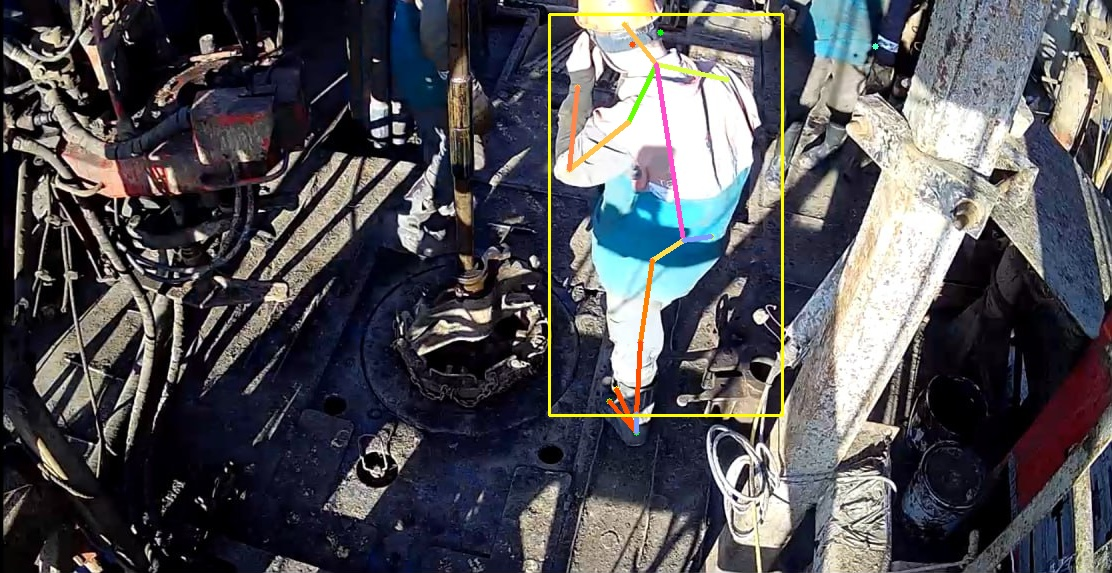
\includegraphics[width=1.0\textwidth,keepaspectratio]{problem_formulation_3}
    \end{figure}
\end{frame}

\begin{frame}
    \frametitle{Постановка задачи}
    Начальные предположения:
    \begin{itemize}
        \item Опасная зона для конкретной камеры задана заранее;
        \item Детектируем только случай нахождения в опасной зоне без СИЗ.
    \end{itemize}

    Список рассматриваемых средств индивидуальной защиты:
    \begin{itemize}
        \item Каска,
        \item Перчатки,
        \item Ботинки.
    \end{itemize}
\end{frame}

\begin{frame}
    \frametitle{Архитектура решения}
    \begin{figure}
        \centering
        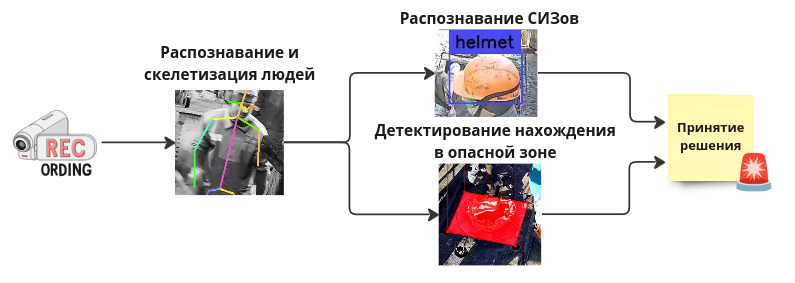
\includegraphics[width=1.1\textwidth,keepaspectratio]{general_architecture}
    \end{figure}
\end{frame}

\begin{frame}
    \frametitle{Цели и задачи}
    Цель работы -- проектирование системы компьютерного зрения для детектирования опасных ситуаций на производстве.

    Задачи работы:
    \begin{enumerate}
        \item Проектирование архитектуры системы компьютерного зрения,
        \item Разработка метода распознавания и скелетизации,
        \item Реализация алгоритма детектирования нахождения в опасной зоне,
        \item Описание принципа принятия решений по заданному кадру.
    \end{enumerate}
\end{frame}


	\section{Распознавание и скелетизация людей}
\begin{frame}
    \frametitle{Распознавание людей и их позиций}
    \begin{figure}
        \centering
        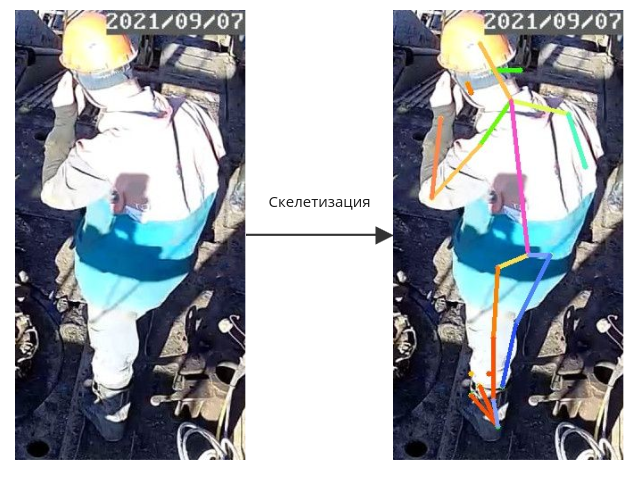
\includegraphics[width=0.9\textwidth,keepaspectratio]{skeletization}
    \end{figure}
\end{frame}

%\begin{frame}
%    \frametitle{Модель AlphaPose}
%    \begin{figure}
%        \centering
%        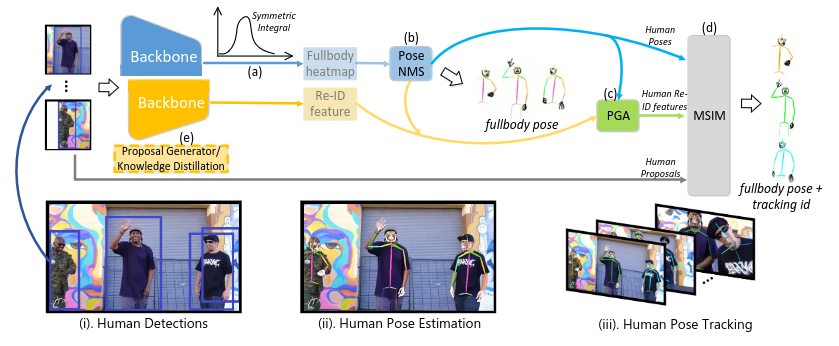
\includegraphics[width=1.0\textwidth,keepaspectratio]{alphapose_1}
%    \end{figure}
%\end{frame}

\begin{frame}
    \frametitle{Модель AlphaPose}
    \begin{figure}
        \centering
        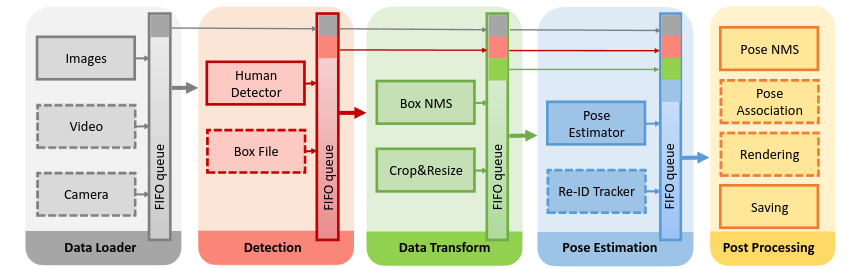
\includegraphics[width=1.0\textwidth,keepaspectratio]{alphapose_2}
    \end{figure}
\end{frame}

\begin{frame}
    \frametitle{Выходной формат данных скелетной модели}
    По заданному кадру алгоритм строит множество $\mathbf{S}$ скелетных моделей.

    Каждый элемент $\mathbf{S}$ имеет вид:
    $$ \left(ID, K, BB\right), $$
    где:
    \begin{itemize}
        \item $ID$ -- уникальный идентификатор человека в кадре,
        \item $K$ -- список ключевых точек скелетной модели,
        \item $BB$ -- ограничивающая рамка для изображения человека.
    \end{itemize}
\end{frame}

\begin{frame}
    \frametitle{Формат представления ключевых точек}
    $$ K = [(x_i, y_i, c_i)]_{i=0}^{N-1}, $$
    где
    \begin{itemize}
        \item $(x_i, y_i)$ -- координаты ключевой точки на изображении,
        \item $c_i$ -- мера уверенности алгоритма, что ключевая точка предсказана корректно,
        \item $N$ -- общее число ключевых точек (26~тело, 21~левая~рука, 21~правая~рука).
    \end{itemize}
\end{frame}

\begin{frame}
    \frametitle{Нумерация ключевых точек}
    \begin{figure}
        \begin{minipage}[!h]{0.49\linewidth}
            \centering
            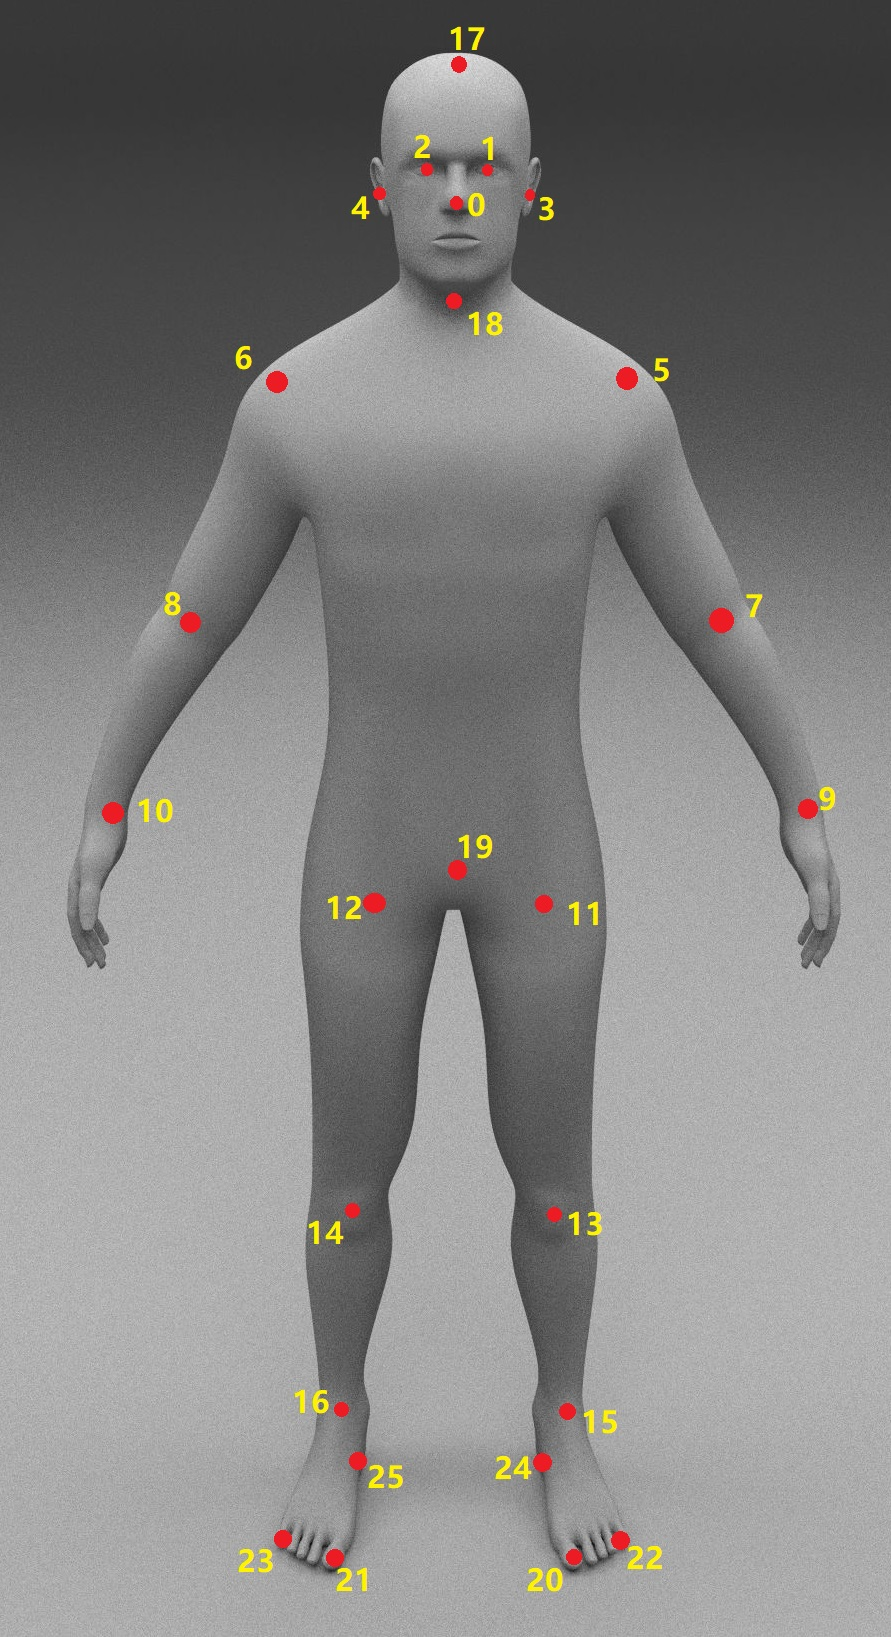
\includegraphics[width=0.7\textwidth,keepaspectratio]{keypoints_map_1}
        \end{minipage}
        \hfill
        \begin{minipage}[!h]{0.49\linewidth}
            \centering
            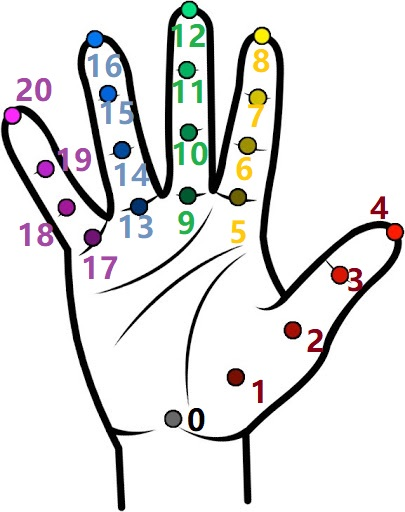
\includegraphics[width=0.7\textwidth,keepaspectratio]{keypoints_map_2}
        \end{minipage}
    \end{figure}
\end{frame}

\begin{frame}
    \frametitle{Рассчет координат и меры уверенности для ключевой точки}
    Пусть $z_{(x, y)}$ --- ненормализованные логиты, выход backbone-части регрессора.

    Определим карту теплоты $C = (c_{(x, y)})$ следующим образом:
    $$ c_{(x, y)} = \sigma (z_{(x, y)})$$

    Мера уверенности для данной точки выражается как:
    $$ conf = \max(C) $$

    Нормализованная карта теплоты $P = (p_{(x, y)})$ выражается следующим образом:
    $$ p_{(x, y)} =  \frac{c_{(x, y)}}{\sum C}$$

\end{frame}

	\section{Детектирование нахождения в опасной зоне}
\begin{frame}
    \frametitle{Простейшее определение опасной зоны}
    В простейшем случае, опасную зону можно определить следующим образом.

    Зафиксируем выпуклый многоугольник $A$ на изображении.
    $$ x_{min} = \min\{ x : \exists y (x, y) \in A\} $$
    $$ x_{max} = \max\{ x : \exists y (x, y) \in A\} $$

    Тогда опасной зоной $DZ$ будем называть выпуклую оболочку множества
    $$ A \cup \{(x_{min}, 0), (x_{max}, 0)\} $$
\end{frame}

\begin{frame}
    \frametitle{Определение принадлежности опасной зоне}
    Задан минимальный порог срабатывания $m$ для принадлежности ключевой точки зоне.

    По определению $I_i = 1$, если ключевая точка человека $\left(x_i, y_i, c_i\right)$ находится в опасной зоне.
    $$ I_i = 1 \iff \left(c_i \ge m\right) \wedge \left(\left(x_i, y_i\right) \in DZ\right) $$

    Задана минимальная доля $t$ ключевых точек, принадлежащих опасной зоне, при которой считаем человека находящимся в ней.

    Считаем, что человек находится в опасной зоне, если:
    $$ \frac{\sum I_i}{N} \ge t $$
\end{frame}

\begin{frame}
    \frametitle{Усложнение определения опасной зоны}
    Будем считать, что область пространства, обозреваемого камерой, локально представляет из себя $\mathbb{R}^3$.

    Зафиксируем правильный многоугольник $A$ в плоскости $z = 0$.
    Тогда опасной зоной будем называть множество:
    $$DZ = \{(x, y, z) : (x, y, 0) \in A\} $$
\end{frame}

\begin{frame}
    \frametitle{Детектирование нахождения в опасной зоне}
    \begin{figure}
        \centering
        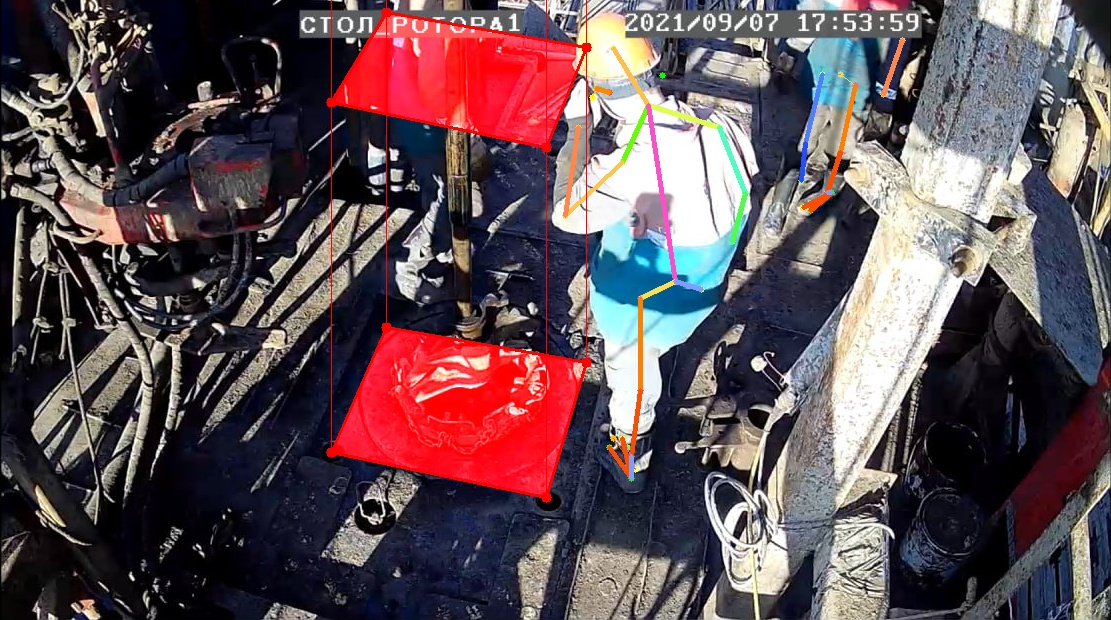
\includegraphics[width=1.0\textwidth,keepaspectratio]{danger_zone}
    \end{figure}
\end{frame}

\begin{frame}
    \frametitle{Оценка расстояния до объектов}
    Рассмотренные подходы к оценке расстояния до объектов:
    \begin{itemize}
        \item Калибровка камеры;
        \item Анализ геометрии помещения;
        \item Аппроксимация карты глубины.
    \end{itemize}
\end{frame}

\begin{frame}
    \frametitle{Карта глубины}
    \begin{definition}
        Карта глубины --- это изображение, где для каждого пикселя вместо цвета хранится расстояние от него до камеры.
    \end{definition}

    \begin{figure}
        \begin{minipage}[!h]{0.49\linewidth}
            \centering
            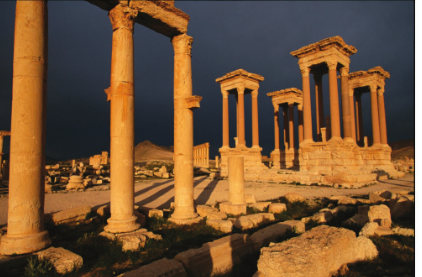
\includegraphics[width=1.0\textwidth,keepaspectratio]{depth_map_example_1}
        \end{minipage}
        \hfill
        \begin{minipage}[!h]{0.49\linewidth}
            \centering
            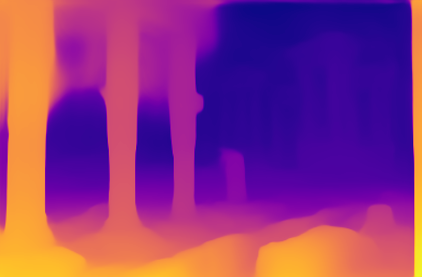
\includegraphics[width=1.0\textwidth,keepaspectratio]{depth_map_example_2}
        \end{minipage}
        \caption{Пример карты глубины, построенной по изображению}
    \end{figure}

\end{frame}

\begin{frame}
    \frametitle{Трёхмерная реконструкция по карте глубины}
    \begin{figure}
        \centering
        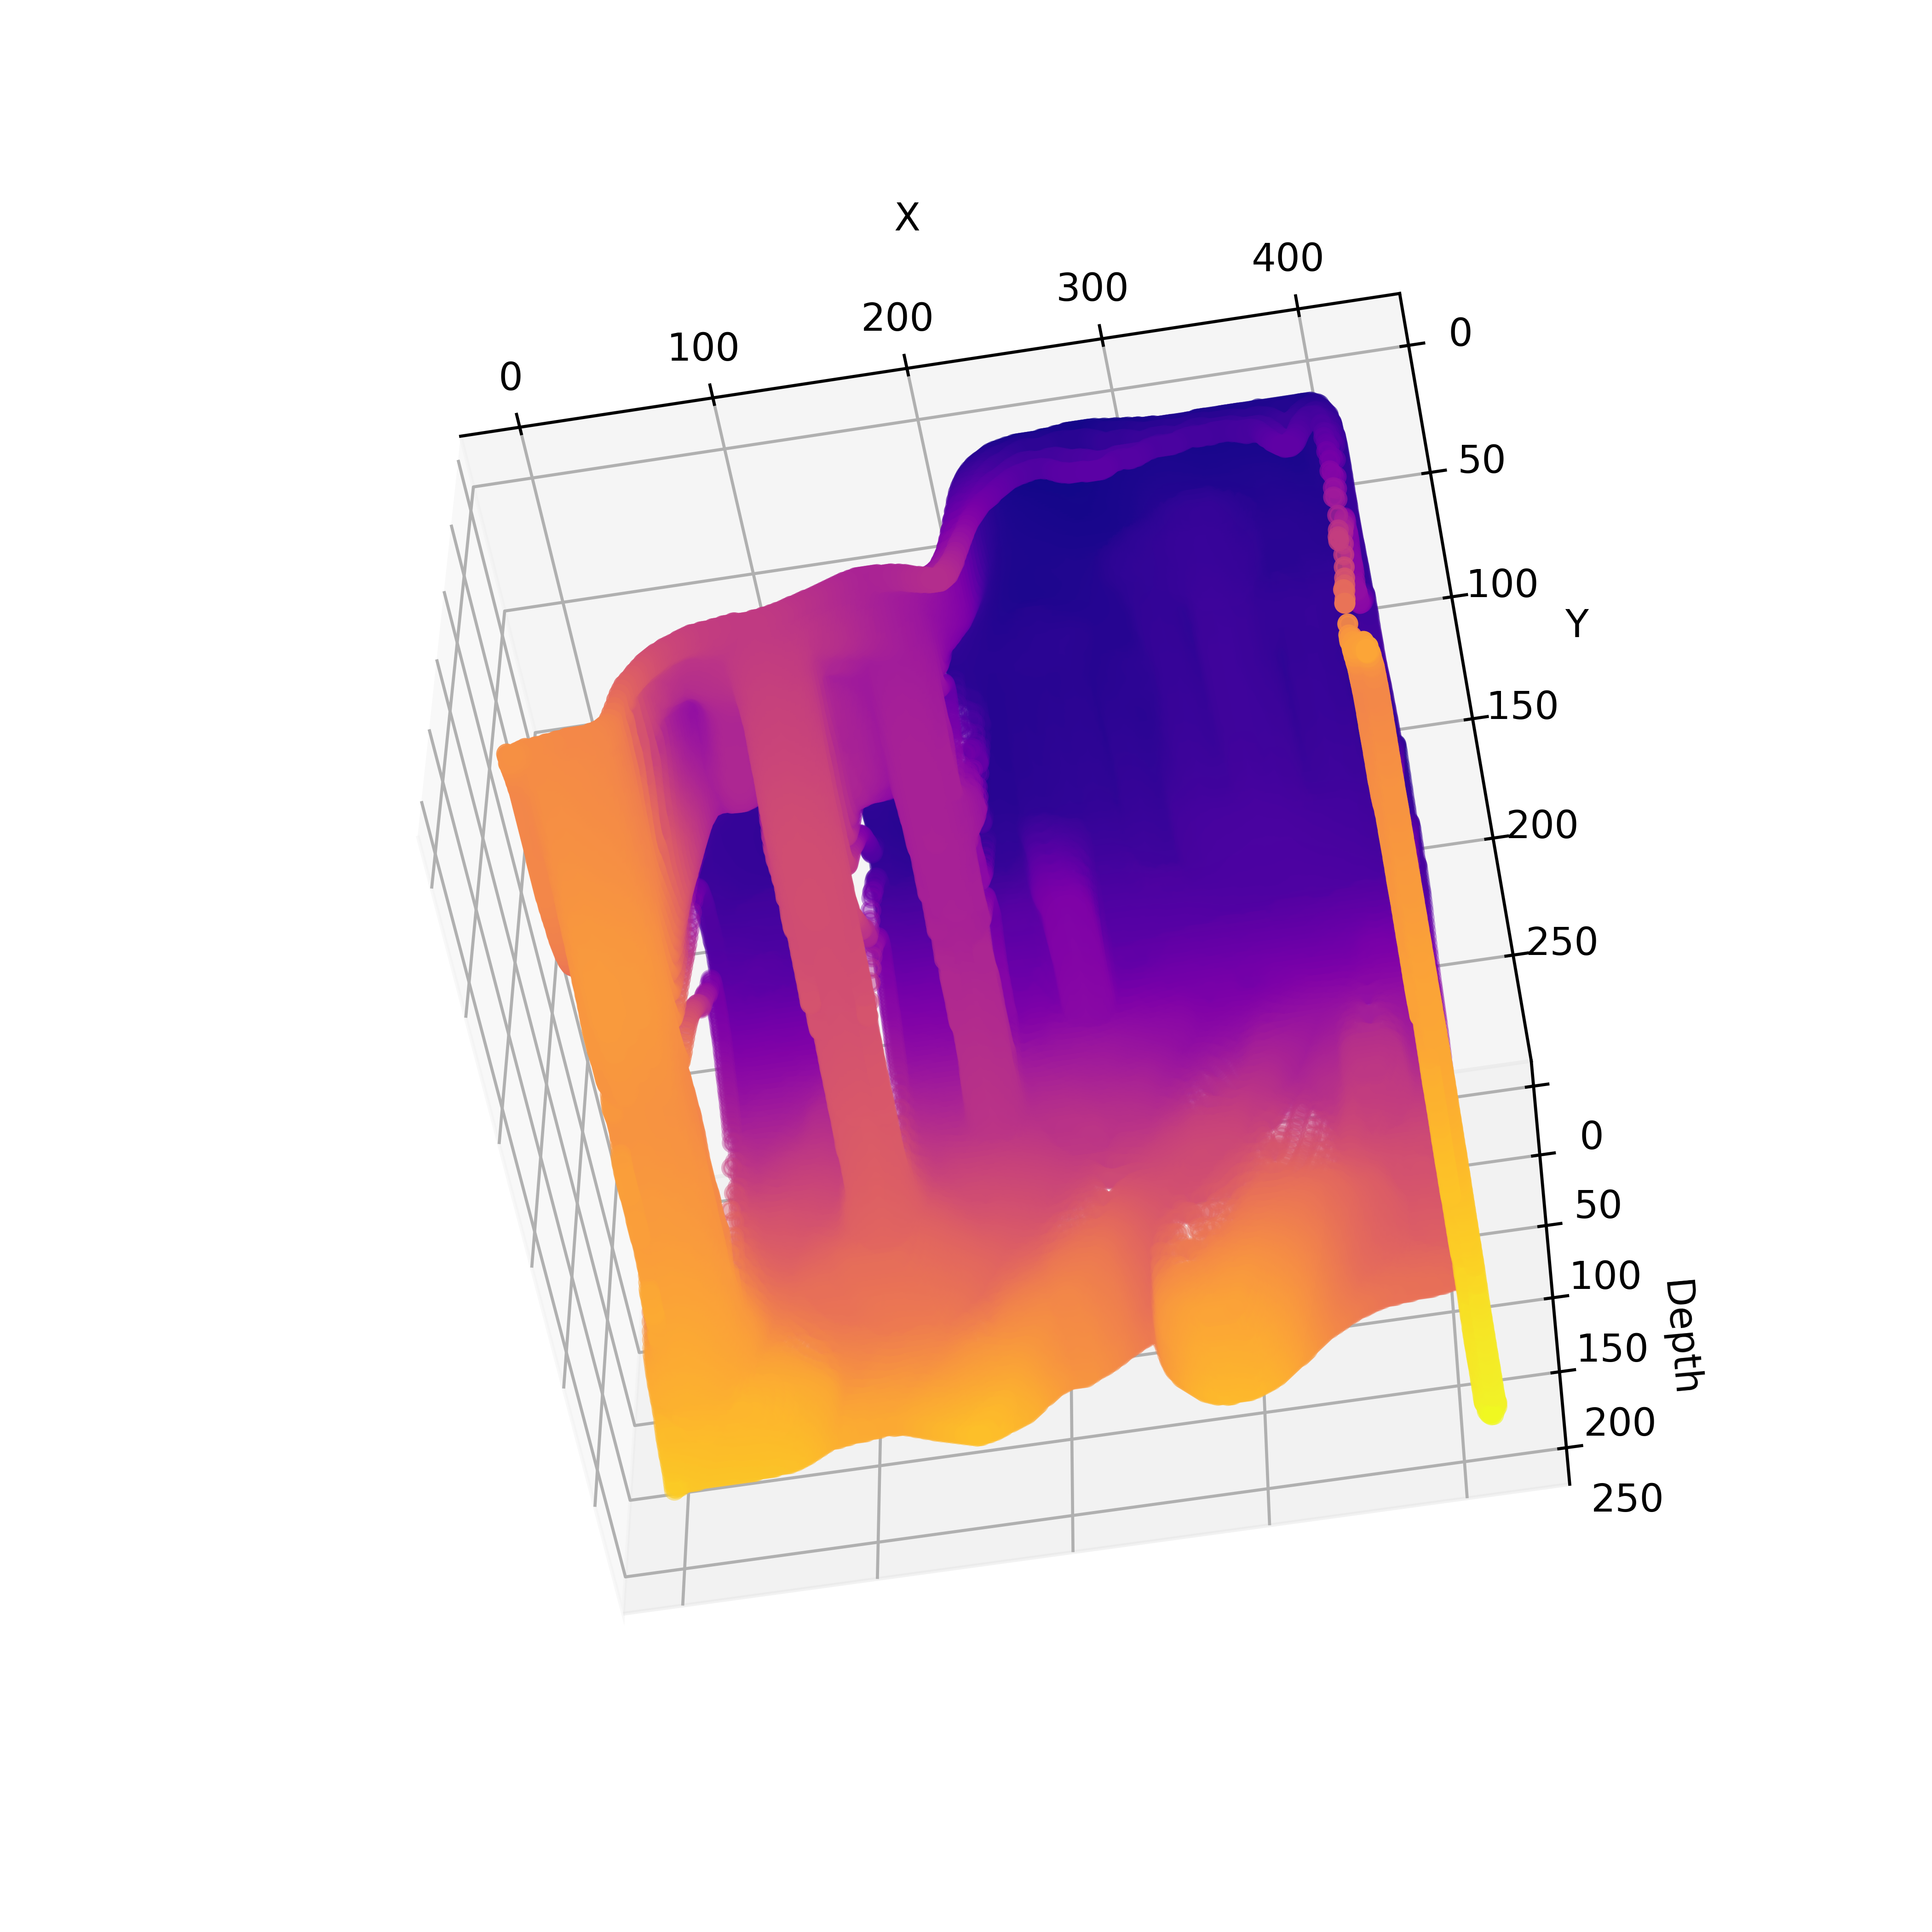
\includegraphics[width=0.8\textwidth,keepaspectratio]{depth_map_example_3}
    \end{figure}
\end{frame}

\begin{frame}
    \frametitle{Модель MiDaS}
    \begin{figure}
        \centering
        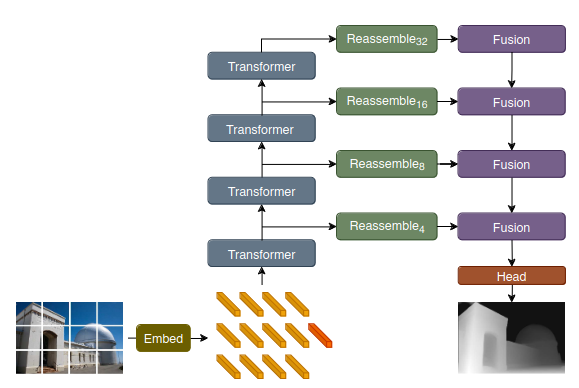
\includegraphics[scale=0.5]{midas}
    \end{figure}
\end{frame}

\begin{frame}
    \frametitle{Получение карты абсолютной глубины}
    Модель Midas строит по изображению карту относительной глубины $M_r$. Преобразуем её в карту абсолютной глубины $M_a$.

    Зная точное расстояние $d_0$ до одной из точек $(x_0, y_0)$ на изображении можно масштабировать карту относительной глубины следующим образом:
    $$ M_a = c \cdot M_r, $$

    где $c = \frac{d}{M_r[x_0, y_0]}$
\end{frame}

\begin{frame}
    \frametitle{Уточнение карты абсолютной глубины}
    Пусть мы знаем расстояния $d = \left(d_0, \dots, d_{k - 1}\right)$ до точек $A = \left((x_0, y_0), \dots, (x_{k - 1}, y_{k - 1})\right)$.

    Определим функцию ошибки приближения следующим образом:
    $$ L_{(d, A)}(c) = \sum\limits_{i = 0}^{k - 1} \left(c \cdot M_r[x_i, y_i] - d_i\right)^2 $$

    Методом наименьших квадратов найдём такое $c$, при котором достигается минимум $L(c)$.
\end{frame}

\begin{frame}
    \frametitle{Примеры работы алгоритма проверки принадлежности опасной зоне}
    \begin{figure}
        \begin{minipage}[!h]{0.49\linewidth}
            \centering
            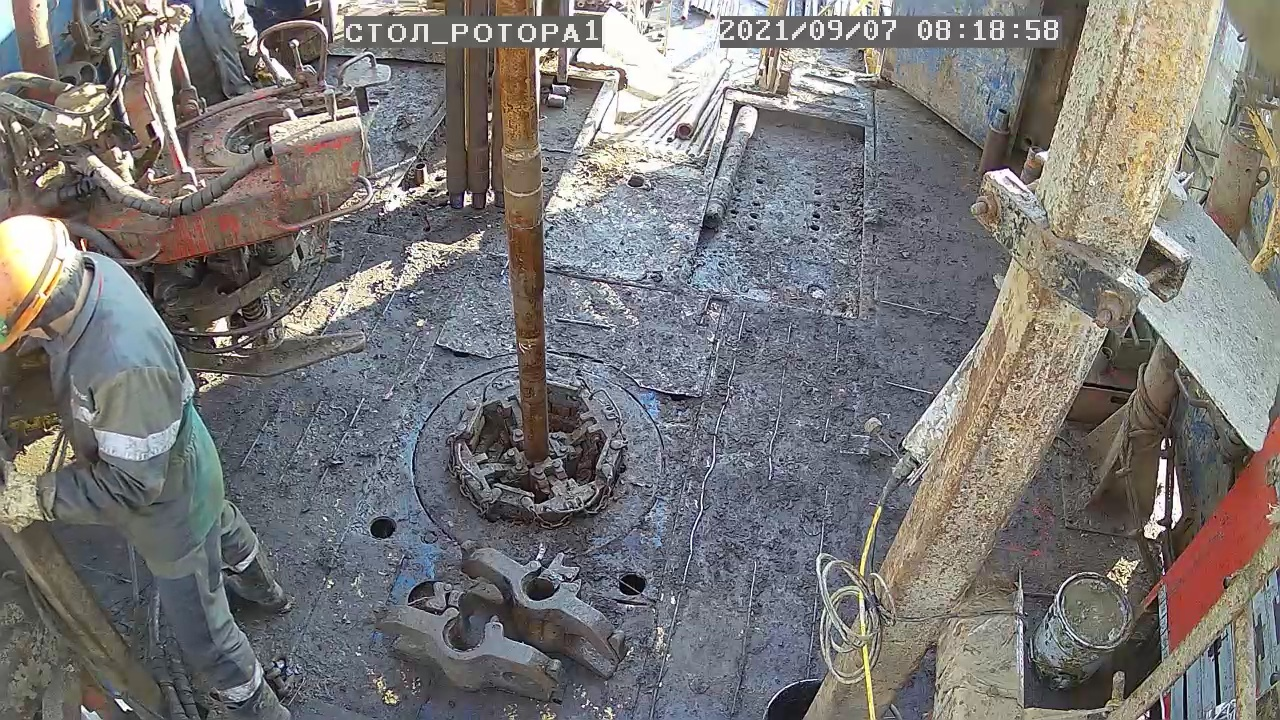
\includegraphics[width=1.0\textwidth,keepaspectratio]{example_1_image}
        \end{minipage}
        \hfill
        \begin{minipage}[!h]{0.49\linewidth}
            \centering
            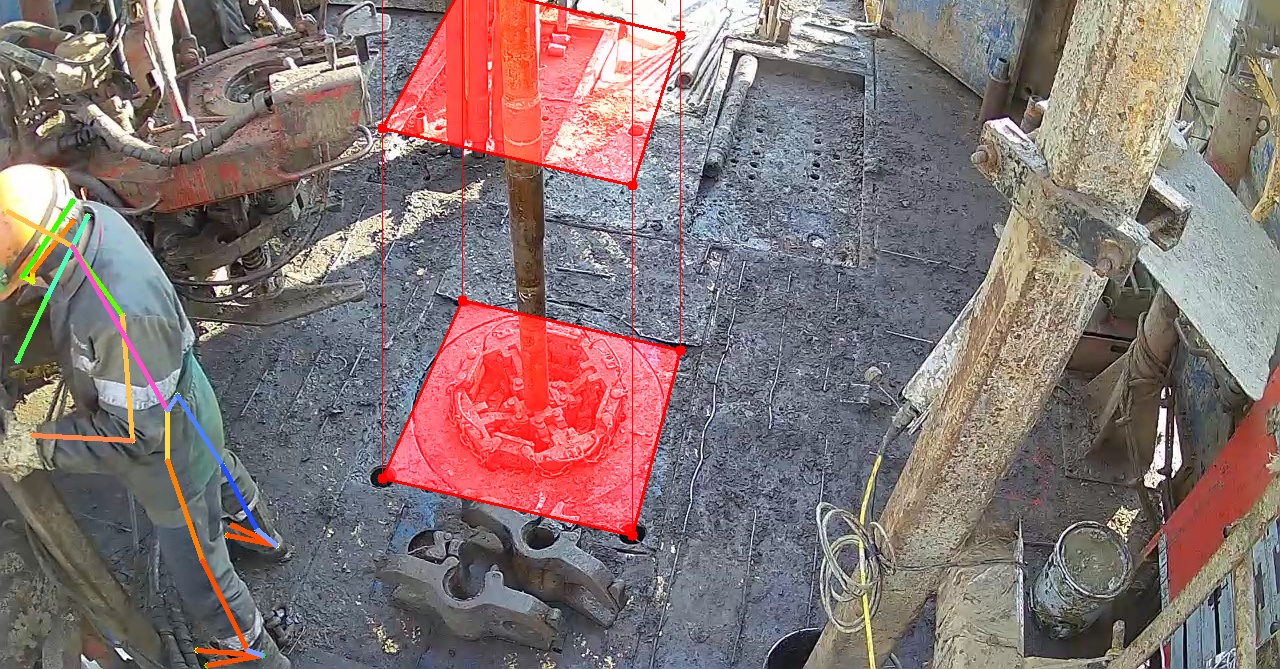
\includegraphics[width=1.08\textwidth,keepaspectratio]{example_1_highlighted}
        \end{minipage}
        \caption{Рабочий в СИЗ не в опасной зоне}
    \end{figure}
\end{frame}

\begin{frame}
    \frametitle{Примеры работы алгоритма проверки принадлежности опасной зоне}
    \begin{figure}
        \begin{minipage}[!h]{0.49\linewidth}
            \centering
            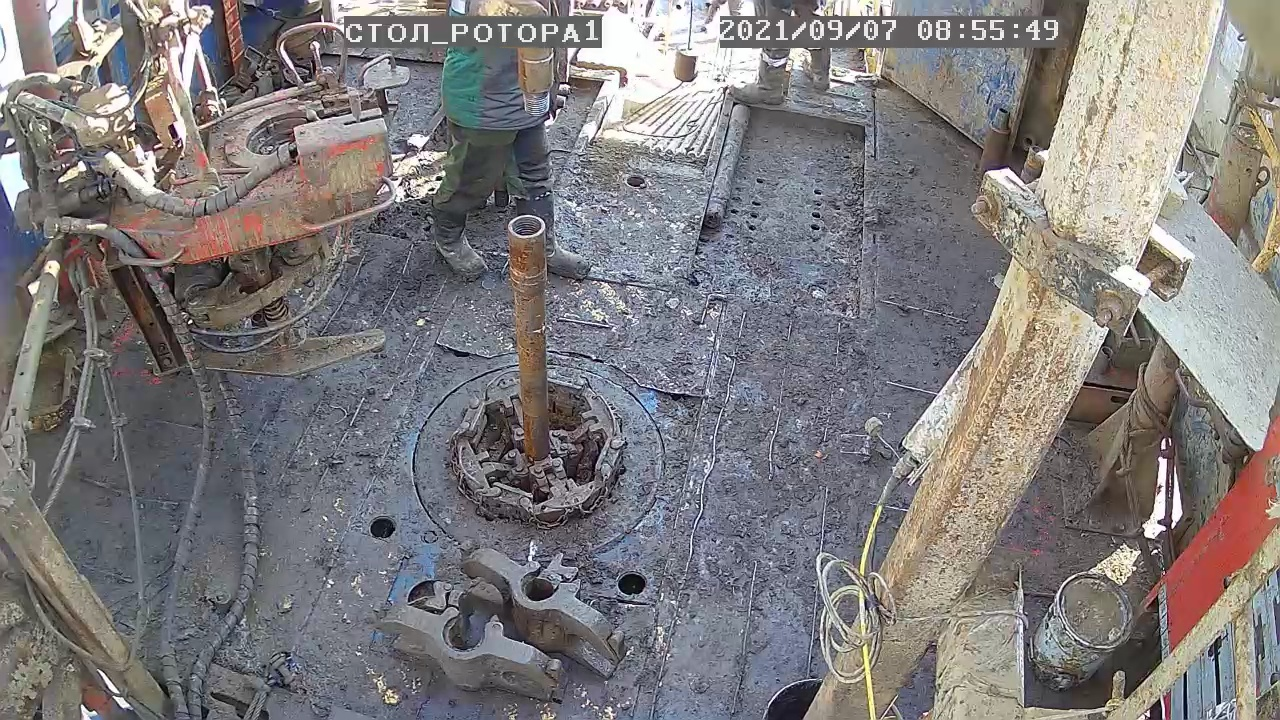
\includegraphics[width=1.0\textwidth,keepaspectratio]{example_2_image}
        \end{minipage}
        \hfill
        \begin{minipage}[!h]{0.49\linewidth}
            \centering
            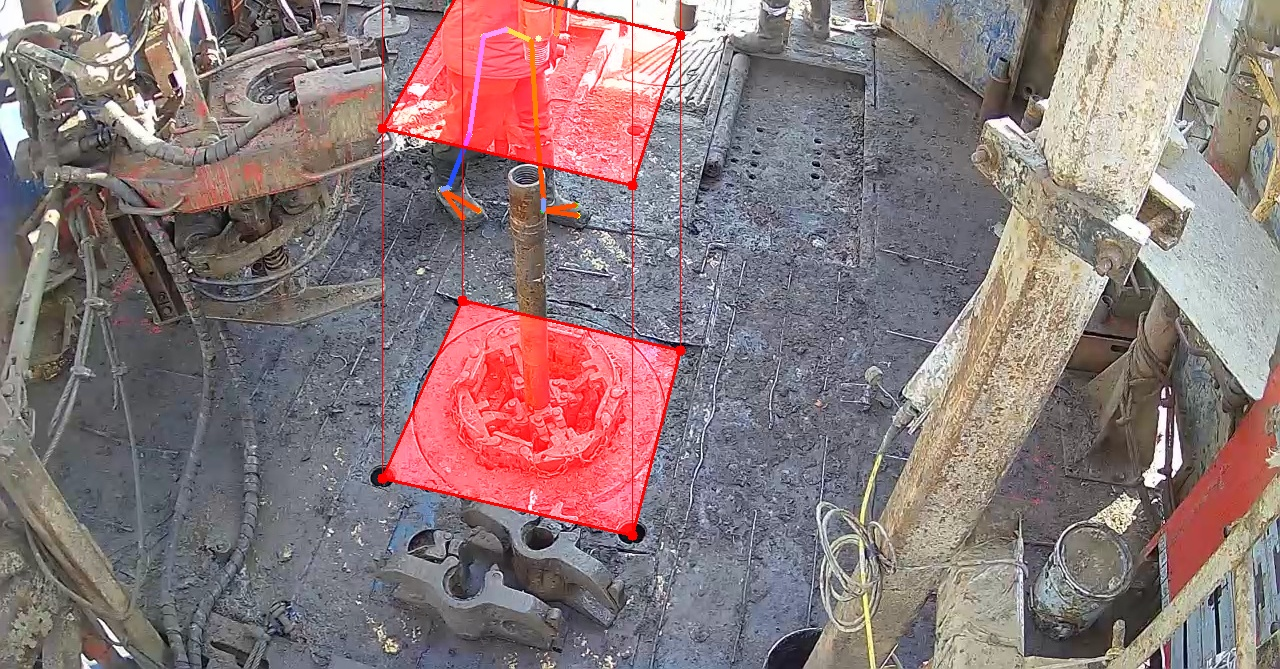
\includegraphics[width=1.08\textwidth,keepaspectratio]{example_2_highlighted}
        \end{minipage}
        \caption{Рабочий в СИЗ за опасной зоной}
    \end{figure}
\end{frame}

\begin{frame}
    \frametitle{Примеры работы алгоритма проверки принадлежности опасной зоне}
    \begin{figure}
        \begin{minipage}[!h]{0.49\linewidth}
            \centering
            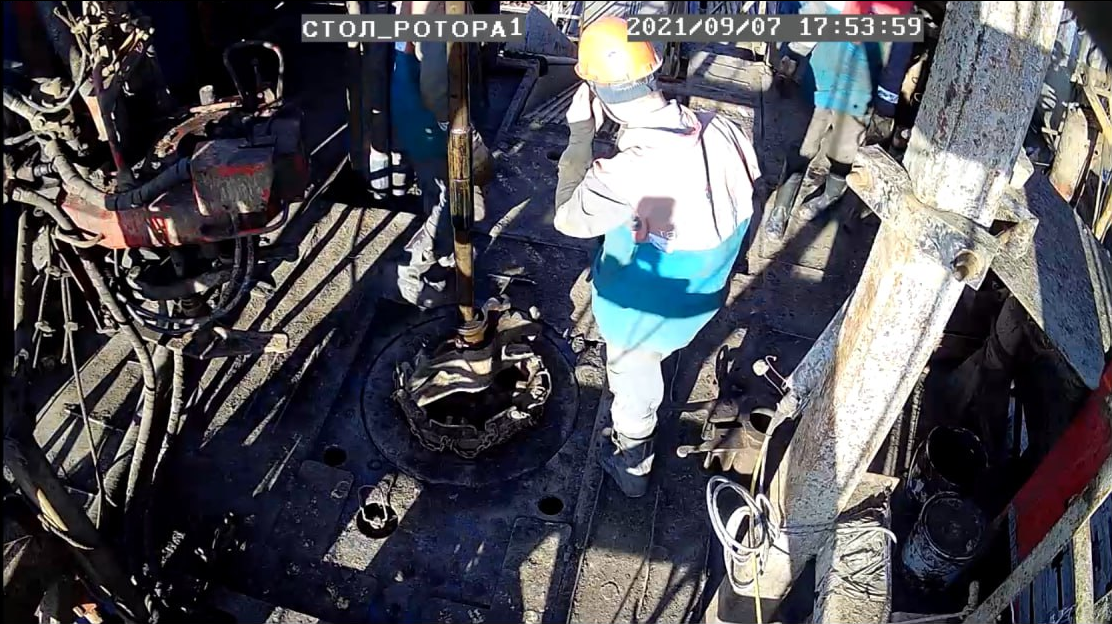
\includegraphics[width=1.0\textwidth,keepaspectratio]{example_3_image}
        \end{minipage}
        \hfill
        \begin{minipage}[!h]{0.49\linewidth}
            \centering
            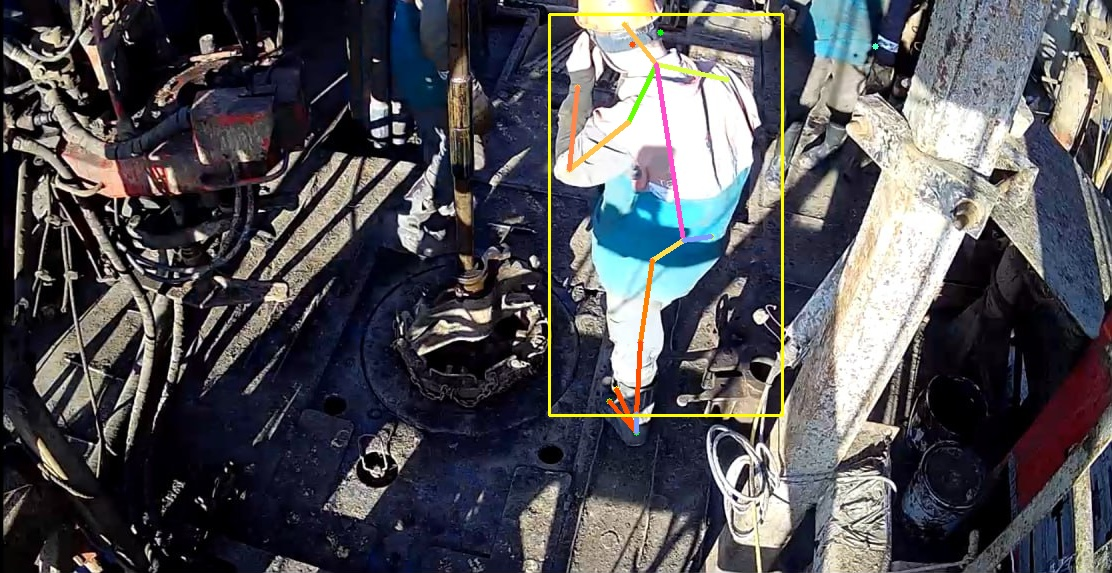
\includegraphics[width=1.08\textwidth,keepaspectratio]{example_3_highlighted}
        \end{minipage}
        \caption{Рабочий без СИЗ в опасной зоне}
    \end{figure}
\end{frame}

    \section{Принятие решения}
\begin{frame}
    \frametitle{Принятие решения}
    Пусть

    $\left[P_i\right]_{i=0}^{M-1}$ -- результат работы модуля распознавания СИЗов,

    $\left[D_i\right]_{i=0}^{M-1}$ -- результат работы модуля детектирования нахождения в опасной зоне:
    $$ P_i = 1 \iff  \text{i-й человек находится в кадре без СИЗ}$$
    $$ D_i = 1 \iff \text{i-й человек находится в кадре в опасной зоне} $$

    В данном случае $M$ -- число обнаруженных людей в кадре.

    Тогда будем считать ситуацию на текущем кадре опасной, если истинно следующее значение:
    $$ F = \bigvee\limits_{i=0}^{M-1} \left(P_i \wedge D_i\right) $$
\end{frame}

\begin{frame}
    \frametitle{Матрица возможных ответов}
    Для расширения спектра возможных ответов требуется введение индикатора присутствия человека без СИЗ в кадре:
    $$ P = \bigvee\limits_{i=0}^{M-1} P_i $$

    \begin{table}
        \centering
        \begin{tabular}{|c|c|c|}
            \hline
            \diagbox{$D_i$}{$P_i$} & $0$ & $1$\\
            \hline
            $0$ & \cellcolor{green}-- & \cellcolor{yellow}$P \wedge \neg F$ \\
            \hline
            $1$ & \cellcolor{green}-- & \cellcolor{red}$F$ \\
            \hline
        \end{tabular}
    \end{table}

\end{frame}

    \section{Результаты}
\begin{frame}
    \frametitle{Результаты}
    \begin{itemize}
        \item Спроектирована архитектура системы компьютерного зрения для детектирования опасных ситуаций на производстве;
        \item Разработан метод построения скелетных представлений людей в кадре с использованием модели AlphaPose;
        \item Реализован алгоритм детектирования принадлежности скелетного представления опасной зоне с использованием модели MiDaS;
        \item Описана принцип принятия решений по заданному кадру.
    \end{itemize}
\end{frame}


    \section{Направления улучшения}
\begin{frame}
    \frametitle{Возможные направления дальнейшего улучшения}
    \begin{itemize}
        \item Калибровка гиперпараметров модели AlphaPose для увеличения стабильности получаемых скелетных моделей
        \item Доработка метода проверки принадлежности опасной зоне на основе поиска калибровочной матрицы
        \item Реализация метода аппроксимации калибровочной матрицы на основе обучения с подкреплением и сравнение его с классическими
        \item Реализация межкадрового взаимодействия блоков для увеличения точности
    \end{itemize}
\end{frame}


\end{document}
